\documentclass{beamer}
\usepackage{amsmath}
\usepackage{tikz}
\usepackage[T1]{fontenc}
\usepackage{lmodern} % Better font support
\usepackage{libertinus} % Libertinus has sans + small caps
\renewcommand{\familydefault}{\sfdefault}
\usepackage{amsmath, amssymb}
\usetikzlibrary{graphs, graphs.standard}
\usepackage{xcolor}
\usepackage{verbatim}
\usepackage{algorithm, algpseudocode} % Use algpseudocode for \Procedure, etc.

% Theme
\usetheme{Madrid}
\usepackage{xcolor}

% Customizing colors
\definecolor{myred}{RGB}{180, 0, 0}
\definecolor{darkred}{RGB}{120, 0, 0}
\setbeamercolor{structure}{fg=myred}
\setbeamercolor{frametitle}{fg=white, bg=myred}
\setbeamercolor{title}{fg=white, bg=myred}
\setbeamercolor{block title}{fg=white, bg=darkred}
\setbeamercolor{block body}{fg=black, bg=white}

% Title Page
\title{Graph Theory and Algorithms}
\subtitle{Lecture 11: Graph Representations and Properties}
\author{Instructor: Dr. Mudassir Shabbir}
\institute{ITU}
\date{February 26, 2025}

\titlegraphic{\hfill
\includegraphics[width=1cm]{Itu.jpg}}

\begin{document}

\begin{frame}
    \titlepage
    \vspace{1cm}
    \textbf{Scribe:} Safwan Ahmad \& Shariq Shoaib
\end{frame}

% Slide: Graph Definition
\begin{frame}{Graph Definition}
    \textbf{Definition:} A graph is a pair of two sets $G(V,E)$ where:
    \begin{itemize}
        \item $V$ is the set of vertices.
        \item $E$ is the set of edges, a subset of $V \times V$.
    \end{itemize}
    
    \textbf{Graph means:}
    \begin{itemize}
        \item \textbf{Undirected}: Edges have no direction.
        \item \textbf{Unweighted}: Edges have no weights.
        \item \textbf{Simple}: No multiple edges or loops.
    \end{itemize}

    \textbf{Types of Graphs:}
    \begin{itemize}
        \item \textbf{Directed Graph}: $(u,v) \in E \neq (v,u) \in E$. (e.g., Twitter)
        \item \textbf{Undirected Graph}: $(u,v) \in E = (v,u) \in E$. (e.g., Facebook, LinkedIn)
        \item \textbf{Weighted Graph}: Graph with weights on edges, $W: E \to \mathbb{R}$.
        \item \textbf{Simple Graph}: No multiple edges or loops.
    \end{itemize}
\end{frame}

% Slide: Connectivity of Graph
\begin{frame}{Connectivity of Graph}
    \textbf{Example Graph:}
    \begin{center}
        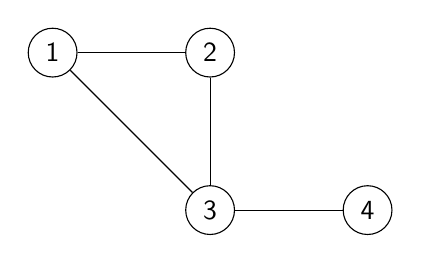
\begin{tikzpicture}
            \node[circle, draw] (1) at (0,0) {1};
            \node[circle, draw] (2) at (2,0) {2};
            \node[circle, draw] (3) at (2,-2) {3};
            \node[circle, draw] (4) at (4,-2) {4};
            \draw (1) -- (2);
            \draw (1) -- (3);
            \draw (2) -- (3);
            \draw (3) -- (4);
        \end{tikzpicture}
        
        \vspace{0.3em}
        \textbf{Figure 1}
    \end{center}
    
    \textbf{Connectivity of Graph:} A graph is connected if every pair of vertices has a path.
    \begin{itemize}
        \item If $(u,v) \in E$, then $u$ and $v$ are \textbf{Adjacent} or \textbf{Incident}.
        \item Every consecutive pair in a walk is adjacent.
    \end{itemize}
\end{frame}

% Slide: Walk
\begin{frame}{Walk}
    \textbf{Walk:} A walk in a graph is a sequence of vertices and edges where both edges and vertices can be repeated.
    \begin{itemize}
        \item Formally, $\langle V_1, V_2, V_3, \dots, V_k \rangle$ where $(V_i, V_{i+1}) \in E$.
        \item \textbf{Example:} in Figure 1 $\langle 1, 2, 3, 4 \rangle$ is a walk.
        \item \textbf{Non-Example:} in Figure 1 $\langle 1, 4 \rangle$ is not a walk (no direct edge).
    \end{itemize}
    \textbf{Key points to note about a walk:}
    \begin{itemize}
        \item Edges can be repeated.
        \item Vertices can be repeated.
    \end{itemize} \
\end{frame}

% Slide: Path and Simple Path
\begin{frame}{Path and Simple Path}
    \textbf{Path:} A walk with no repeated edges.
    \begin{itemize}
        \item \textbf{Example:} in Figure 1 $\langle 1, 2, 3 \rangle$ is a path.
    \end{itemize}

    \textbf{Simple Path:} a path in a graph which does not have repeating vertices.
    \begin{itemize}
        \item \textbf{Example:} in Figure 1 $\langle 1, 2, 3 \rangle$ is a simple path.
    \end{itemize}
\end{frame}

% Slide: Length of a Path
\begin{frame}{Length of a Path}
    \textbf{Definition:} For a path $P = \langle v_1, v_2, \dots, v_k \rangle$, the length is the number of edges involved.
    \begin{itemize}
        \item Length $l = k - 1$, where $k$ is the total number of vertices.
    \end{itemize}

    \textbf{Examples:}
    \begin{itemize}
        \item $\langle 1, 4 \rangle$ has length $l = 1$ (1 edge).
        \item $\langle 1 \rangle$ has length $l = 0$ (no edges).
    \end{itemize}
\end{frame}

% Slide: Shortest Path (Smaller Graph)
\begin{frame}{Shortest Path}
    \textbf{Shortest Path:}
    \begin{itemize}
        \item For an \textbf{unweighted graph}, the shortest path is the path from $v_1$ to $v_k$ with the minimum number of edges.
        \item \textbf{Example:} In Figure 1, the shortest path from vertex 1 to vertex 4 is $\langle 1, 3, 4 \rangle$ with 2 edges.
        \vspace{1em}
        \item For a \textbf{weighted graph}, the shortest path is the path from $v_1$ to $v_k$ where the sum of edge weights is minimized.
        \item \textbf{Example:} Suppose the weights on the edges in Figure 1 are:
        \begin{itemize}
            \item (1,2): 3, (1,3): 1, (2,3): 1, (3,4): 2
        \end{itemize}
        Then the shortest path from vertex 1 to vertex 4 is $\langle 1, 3, 4 \rangle$ with total weight $1 + 2 = 3$.
    \end{itemize}
\end{frame}

% Slide: Cycle, Simple Cycle
\begin{frame}{Cycle, Simple Cycle}
    \textbf{Cycle:} A path where the first and last vertex are the same.
    \begin{itemize}
        \item \textbf{Example:} in Figure 1 $\langle 1, 2, 3, 1 \rangle$ is a cycle.
    \end{itemize}

    \textbf{Simple Cycle:} A simple path where the first and last vertex are the same.
    \begin{itemize}
        \item \textbf{Example:} in Figure 1 $\langle 1, 2, 3, 1 \rangle$ is a simple cycle.
    \end{itemize}\
\end{frame}

% Slide: Forest
\begin{frame}{Forest}
    \textbf{Forest:} A forest is a graph with no cycles.
    \begin{itemize}
        \item A forest can consist of multiple disconnected trees.
        \item \textbf{Example:} The graph below is a forest with two trees.
    \end{itemize}

    \centering
    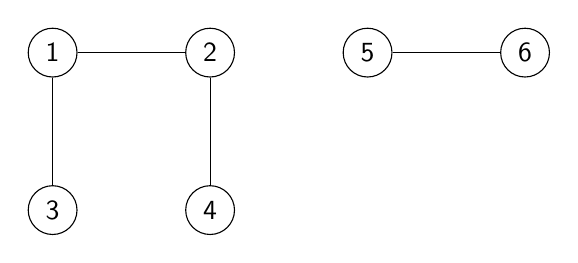
\begin{tikzpicture}
        \node[circle, draw] (1) at (0,0) {1};
        \node[circle, draw] (2) at (2,0) {2};
        \node[circle, draw] (3) at (0,-2) {3};
        \node[circle, draw] (4) at (2,-2) {4};
        \node[circle, draw] (5) at (4,0) {5};
        \node[circle, draw] (6) at (6,0) {6};
        \draw (1) -- (2);
        \draw (1) -- (3);
        \draw (2) -- (4);
        \draw (5) -- (6);
    \end{tikzpicture}
\end{frame}

% Slide: Connected
\begin{frame}{Connected}
    \textbf{Connected:}
    \begin{itemize}
        \item Two vertices $u, v \in V$ are connected if there is a walk from $u$ to $v$.
        \item A graph $G$ is connected if every pair of vertices $u, v \in V$ is connected.
        \item \textbf{Key Points:}
            \begin{itemize}
                \item If there is an edge between two vertices, they are connected and adjacent.
                \item If a path exists between two vertices, they are connected but not necessarily adjacent.
                \item They are adjacent only if there is a direct edge between them.
            \end{itemize}
        \item \textbf{Example:} In the graph below, vertices $2$ and $3$ are connected but not adjacent.
    \end{itemize}

    \centering
    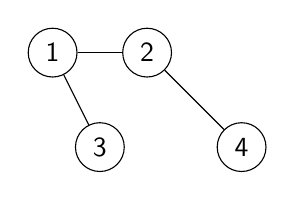
\begin{tikzpicture}[scale=0.8]
        \node[circle, draw] (1) at (0,0) {1};
        \node[circle, draw] (2) at (1.5,0) {2};
        \node[circle, draw] (3) at (0.75,-1.5) {3};
        \node[circle, draw] (4) at (3,-1.5) {4};
        \draw (1) -- (2);
        \draw (1) -- (3);
        \draw (2) -- (4);
    \end{tikzpicture}
\end{frame}


% Slide: Tree and Examples
\begin{frame}{Tree and Examples}
    \textbf{Tree:} A tree is a connected forest.
    \begin{itemize}
        \item A tree is a connected graph with no cycles.
        \item \textbf{Example:} The graph below is a tree.
    \end{itemize}

    \centering
    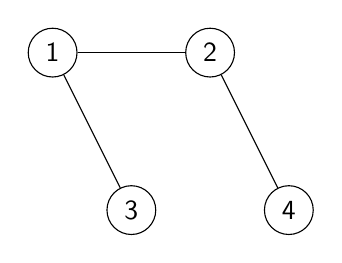
\begin{tikzpicture}
        \node[circle, draw] (1) at (0,0) {1};
        \node[circle, draw] (2) at (2,0) {2};
        \node[circle, draw] (3) at (1,-2) {3};
        \node[circle, draw] (4) at (3,-2) {4};
        \draw (1) -- (2);
        \draw (1) -- (3);
        \draw (2) -- (4);
    \end{tikzpicture}

    \textbf{Additional Examples:}
    \begin{itemize}
        \item \textbf{Connected but Not Adjacent:} In the tree above, vertices $1$ and $4$ are connected (path: $\langle 1, 2, 4 \rangle$) but not adjacent.
        \item \textbf{Adjacent and Connected:} In the tree above, vertices $1$ and $2$ are both connected and adjacent.
    \end{itemize}
\end{frame}

% Slide: Neighbours and Degrees
\begin{frame}{Neighbours and Degrees}
    \textbf{Definition:} If $(u, v) \in E$, then $v$ is a neighbour of $u$.
    \begin{itemize}
        \item For directed graphs, $(u, v) \in E$ means $v$ is an out-neighbour of $u$ and $u$ is an in-neighbour of $v$.
        \item $N(u) = \{v: (u,v) \in E\}$
        \item $|N(u)| = d(u)$, where $d(u)$ is the degree of $u$.
    \end{itemize}

    \centering
    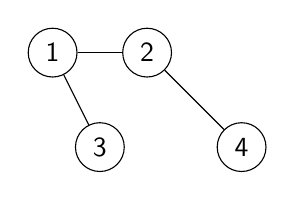
\begin{tikzpicture}[scale=0.8]
        \node[circle, draw] (1) at (0,0) {1};
        \node[circle, draw] (2) at (1.5,0) {2};
        \node[circle, draw] (3) at (0.75,-1.5) {3};
        \node[circle, draw] (4) at (3,-1.5) {4};
        \draw (1) -- (2);
        \draw (1) -- (3);
        \draw (2) -- (4);
    \end{tikzpicture}

    \begin{itemize}
        \item $N(1) = \{2, 3\}$ and $d(1) = 2$.
        \item $N(2) = \{1, 4\}$ and $d(2) = 2$.
        \item $N(3) = \{1\}$ and $d(3) = 1$.
        \item $N(4) = \{2\}$ and $d(4) = 1$.
    \end{itemize}
\end{frame}

% Slide: MST Graph
\begin{frame}{Representation}
    \textbf{MST Graph:}
    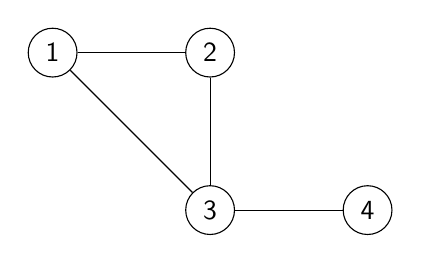
\begin{tikzpicture}
        \node[circle, draw] (1) at (0,0) {1};
        \node[circle, draw] (2) at (2,0) {2};
        \node[circle, draw] (3) at (2,-2) {3};
        \node[circle, draw] (4) at (4,-2) {4};
        \draw (1) -- (2);
        \draw (1) -- (3);
        \draw (2) -- (3);
        \draw (3) -- (4);
    \end{tikzpicture}
    \begin{itemize}
        \item Nodes: 1, 2, 3, 4
    \end{itemize}
\end{frame}

% Slide: Adjacency List
\begin{frame}{Adjacency List}
    \textbf{Adjacency List:}
    \begin{center}
        \begin{tabular}{|c|c|}
            \hline
            \textbf{Vertex} & \textbf{Adjacent Vertices} \\
            \hline
            1 & 2, 3 \\
            2 & 1, 3 \\
            3 & 1, 2, 4 \\
            4 & 3 \\
            \hline
        \end{tabular}
    \end{center}
    \textbf{Explanation:}
    \begin{itemize}
        \item Each vertex is listed with its adjacent vertices.
        \item For example, vertex 1 is connected to vertices 2 and 3.
    \end{itemize}
\end{frame}

% Slide: Adjacency Matrix
\begin{frame}{Adjacency Matrix}
    \textbf{Adjacency Matrix:}
    \[
    \begin{bmatrix}
        0 & 1 & 1 & 0 \\
        1 & 0 & 1 & 0 \\
        1 & 1 & 0 & 1 \\
        0 & 0 & 1 & 0 \\
    \end{bmatrix}
    \]
    \textbf{Explanation:}
    \begin{itemize}
        \item Rows and columns represent vertices 1, 2, 3, 4.
        \item A `1` indicates an edge between the corresponding vertices.
        \item For example, the edge between 1 and 2 is represented by a `1` in the first row, second column.
    \end{itemize}
\end{frame}

% Slide: DFS Algorithm (Introduction)
\begin{frame}{DFS Algorithm}
    \textbf{Depth First Search (DFS):}
    \begin{itemize}
        \item DFS is a graph traversal algorithm.
        \item It explores as far as possible along each branch before backtracking.
        \item Used in applications like:
        \begin{itemize}
            \item Pathfinding
            \item Cycle detection
            \item Topological sorting
            \item Solving puzzles and mazes
        \end{itemize}
    \end{itemize}
\end{frame}

% Slide: DFS Algorithm (Steps)
\begin{frame}{DFS Algorithm Steps}
    \textbf{How DFS Works:}
    \begin{itemize}
        \item Start at a source vertex \( V1 \).
        \item Mark \( V1 \) as visited.
        \item For each neighbor \( v \in N(V1) \):
        \begin{itemize}
            \item If \( v \) is not visited, recursively apply DFS to \( v \).
        \end{itemize}
    \end{itemize}
\end{frame}

% Slide: DFS Algorithm (Without Wrapper)
\begin{frame}{DFS Algorithm: Without Wrapper}
    \textbf{Pseudocode for DFS (Connected Graph):}
    \begin{itemize}
        \item Use it when the graph is connected and a single start vertex is sufficient.
        \item Traversal starts from a source node and explores all reachable vertices.
    \end{itemize}

    \begin{algorithmic}[1]
        \Procedure{DFS}{V}
            \State \( V.\text{visited} \gets \text{True} \)
            \For{each neighbor \( u \in N(V) \)}
                \If{\( u.\text{visited} = \text{False} \)}
                    \State \Call{DFS}{u}
                \EndIf
            \EndFor
        \EndProcedure
    \end{algorithmic}
\end{frame}

\begin{frame}{DFS Algorithm: Wrapper Concept}
    \textbf{Pseudocode for DFS (Disconnected Graph):}
    \begin{itemize}
        \item Wrapper function ensures that \textbf{all graph components} are visited.
        \item Used when the graph may have disconnected parts.
    \end{itemize}

    \begin{algorithmic}[1]
        \Procedure{DFS-Wrapper}{Graph G}
            \For{each vertex \( V \in G \)}
                \If{\( V.\text{visited} = \text{False} \)}
                    \State \Call{DFS}{V}
                \EndIf
            \EndFor
        \EndProcedure
    \end{algorithmic}
\end{frame}

\begin{frame}{DFS Algorithm: Recursive DFS Function}
    \textbf{Inner DFS Procedure:}
    \begin{itemize}
        \item Recursively visits all vertices reachable from the starting vertex.
        \item Called by the wrapper for unvisited vertices.
    \end{itemize}

    \begin{algorithmic}[1]
        \Procedure{DFS}{V}
            \State \( V.\text{visited} \gets \text{True} \)
            \For{each neighbor \( u \in N(V) \)}
                \If{\( u.\text{visited} = \text{False} \)}
                    \State \Call{DFS}{u}
                \EndIf
            \EndFor
        \EndProcedure
    \end{algorithmic}
\end{frame}

% Slide: DFS Example – Connected Graph
\begin{frame}{DFS Example – Connected Graph}

    \textbf{Connected Graph:}

    \begin{center}
    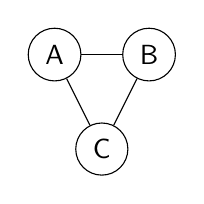
\begin{tikzpicture}[scale=0.8]
        \node[circle, draw] (A) at (0,0) {A};
        \node[circle, draw] (B) at (1.5,0) {B};
        \node[circle, draw] (C) at (0.75,-1.5) {C};
        \draw (A) -- (B);
        \draw (A) -- (C);
        \draw (B) -- (C);
    \end{tikzpicture}
    \end{center}

    \vspace{1em}
    \textbf{DFS Process:}
    \begin{itemize}
        \item Start at A: Visit A $\rightarrow$ B $\rightarrow$ C.
        \item Traversal order may vary depending on neighbor order.
    \end{itemize}
\end{frame}

% Slide: DFS Example – Disconnected Graph
\begin{frame}{DFS Example – Disconnected Graph}

    \textbf{Disconnected Graph:}

    \begin{center}
    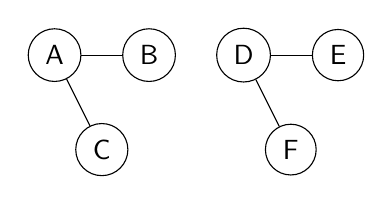
\begin{tikzpicture}[scale=0.8]
        \node[circle, draw] (A) at (0,0) {A};
        \node[circle, draw] (B) at (1.5,0) {B};
        \node[circle, draw] (C) at (0.75,-1.5) {C};
        \node[circle, draw] (D) at (3,0) {D};
        \node[circle, draw] (E) at (4.5,0) {E};
        \node[circle, draw] (F) at (3.75,-1.5) {F};
        \draw (A) -- (B);
        \draw (A) -- (C);
        \draw (D) -- (E);
        \draw (D) -- (F);
    \end{tikzpicture}
    \end{center}

    \vspace{1em}
    \textbf{DFS Process:}
    \begin{itemize}
        \item Start at A: Visit A $\rightarrow$ B $\rightarrow$ C.
        \item Since the graph is disconnected, apply DFS again from D: Visit D $\rightarrow$ E $\rightarrow$ F.
    \end{itemize}
\end{frame}

\begin{frame}{DFS Edge Classifications – Definitions \& Explanations}
    \textbf{Types of Edges in DFS:}
    \begin{itemize}
        \item \textbf{Tree Edge}: An edge \( (u, v) \) where \( v \) is unvisited when \( (u, v) \) is explored.  
        \textcolor{gray}{\small These form the DFS tree and represent discovery of new vertices.}

        \item \textbf{Back Edge}: An edge \( (u, v) \) that connects \( u \) to an ancestor \( v \) in the DFS tree (\( v.\mathrm{visited} = \mathrm{True} \)).  
        \textcolor{gray}{\small Indicates a cycle if the graph is directed.}

        \item \textbf{Forward Edge}: An edge \( (u, v) \) where \( v \) is a descendant of \( u \) in the DFS tree and already visited.  
        \textcolor{gray}{\small Traverses deeper parts of the tree, but not new vertices.}

        \item \textbf{Cross Edge} (optional): An edge \( (u, v) \) that connects nodes in separate branches or components (not ancestor/descendant).  
        \textcolor{gray}{\small Typically occurs in directed graphs during DFS.}
    \end{itemize}
\end{frame}

\begin{frame}{DFS Edge Classifications – Example}
    \textbf{Graph:}
    \begin{center}
    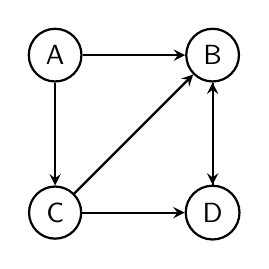
\begin{tikzpicture}[->, >=stealth, node distance=2cm and 2.5cm, thick, scale=1, transform shape]
        % Nodes
        \node[circle, draw] (A) at (0,0) {A};
        \node[circle, draw] (B) at (2,0) {B};
        \node[circle, draw] (C) at (0,-2) {C};
        \node[circle, draw] (D) at (2,-2) {D};

        % Edges
        \draw (A) -> (B);  % Tree Edge
        \draw (B) -> (D);  % Tree Edge
        \draw (A) -> (C);  % Tree Edge
        \draw (D) -> (B);  % Back Edge
        \draw (C) -> (D);  % Forward Edge
        \draw (C) -> (B);  % Cross Edge
    \end{tikzpicture}
    \end{center}

    \textbf{Edge Classifications:}
    \begin{itemize}
        \item \textbf{Tree Edges}: \( (A, B), (B, D), (A, C) \)
        \item \textbf{Back Edge}: \( (D, B) \)
        \item \textbf{Forward Edge}: \( (C, D) \)
        \item \textbf{Cross Edge}: \( (C, B) \)
    \end{itemize}
\end{frame}

% Slide: BFS Algorithm
\begin{frame}{BFS Algorithm}
    \textbf{BFS Algorithm:}
    \begin{itemize}
        \item Start at a vertex \( U \).
        \item Use a queue \( Q \) to manage vertices.
        \item Mark the starting vertex as visited and enqueue it.
        \item While the queue is not empty, dequeue a vertex and explore its neighbors.
        \item Mark and enqueue unvisited neighbors.
    \end{itemize}
\end{frame}

\begin{frame}{BFS Algorithm: Mathematical Form}
    \textbf{Mathematical Form:}
    \begin{algorithmic}[1]
        \Procedure{BFS}{U, Q}
        \State \textbf{for each} vertex $v$ in graph: $v.\text{visited} \gets \text{False}$ \Comment{Initialize visited}
        \State \Call{Push}{U, Q}
        \State $U.\text{visited} \gets \text{True}$
        \While{$ Q \neq \emptyset $}
            \State $ U \gets \Call{Pop}{Q} $
            \For{each neighbor $ Y \in N(U) $}
                \If{$ Y.\text{visited} = \text{False} $}
                    \State $Y.\text{visited} \gets \text{True}$
                    \State \Call{Push}{Y, Q}
                \EndIf
            \EndFor
        \EndWhile
        \EndProcedure
    \end{algorithmic}
\end{frame}

\begin{frame}{BFS Example: Connected Graph}
    \textbf{Connected Graph:}

    \begin{center}
        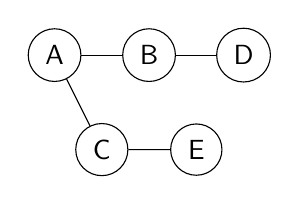
\begin{tikzpicture}[scale=0.8]
            \node[circle, draw] (A) at (0,0) {A};
            \node[circle, draw] (B) at (1.5,0) {B};
            \node[circle, draw] (C) at (0.75,-1.5) {C};
            \node[circle, draw] (D) at (3,0) {D};
            \node[circle, draw] (E) at (2.25,-1.5) {E}; 
            \draw (A) -- (B);
            \draw (A) -- (C);
            \draw (B) -- (D);
            \draw (C) -- (E);
        \end{tikzpicture}
    \end{center}
    
    \textbf{BFS Process:}
    \begin{itemize}
        \item Start at A: Visit A $\rightarrow$ B $\rightarrow$ C $\rightarrow$ D $\rightarrow$ E.
    \end{itemize}
\end{frame}


\begin{frame}{BFS Queue Process} 
    \textbf{Queue Process:}
    \begin{itemize}
        \item Initialize: \( Q = [A] \)
        \item Step 1: Pop A, enqueue B and C. \( Q = [B, C] \)
        \item Step 2: Pop B, enqueue D. \( Q = [C, D] \)
        \item Step 3: Pop C, enqueue E. \( Q = [D, E] \)
        \item Step 4: Pop D. \( Q = [E] \)
        \item Step 5: Pop E. \( Q = [] \)
    \end{itemize}
\end{frame}


% Slide: BFS Tree Edges
\begin{frame}{BFS Tree Edges}
    \textbf{Tree Edges:}
    \begin{itemize}
        \item Tree edges are the edges that connect a vertex to its unvisited neighbors.
        \item In BFS, tree edges always go from a vertex at level \( L \) to a vertex at level \( L+1 \).
        \item Example: A $\rightarrow$ B, A $\rightarrow$ C, B $\rightarrow$ D, C $\rightarrow$ E.
    \end{itemize}

    \centering
    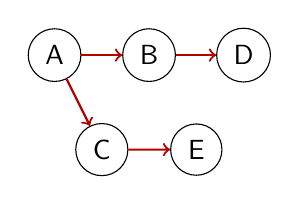
\begin{tikzpicture}[scale=0.8]
        \node[circle, draw] (A) at (0,0) {A};
        \node[circle, draw] (B) at (1.5,0) {B};
        \node[circle, draw] (C) at (0.75,-1.5) {C};
        \node[circle, draw] (D) at (3,0) {D};
        \node[circle, draw] (E) at (2.25,-1.5) {E};
        \draw[->, thick, myred] (A) -- (B); % Tree edge
        \draw[->, thick, myred] (A) -- (C); % Tree edge
        \draw[->, thick, myred] (B) -- (D); % Tree edge
        \draw[->, thick, myred] (C) -- (E); % Tree edge
    \end{tikzpicture}
\end{frame}

% Slide: BFS Cross Edges
\begin{frame}{BFS Cross Edges}
    \textbf{Cross Edges:}
    \begin{itemize}
        \item Cross edges are edges between vertices at the same level.
        \item In BFS, cross edges do not exist in trees but can exist in general graphs.
        \item Example: None in this graph (since it is a tree).
    \end{itemize}

    \centering
    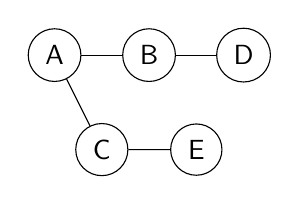
\begin{tikzpicture}[scale=0.8]
        \node[circle, draw] (A) at (0,0) {A};
        \node[circle, draw] (B) at (1.5,0) {B};
        \node[circle, draw] (C) at (0.75,-1.5) {C};
        \node[circle, draw] (D) at (3,0) {D};
        \node[circle, draw] (E) at (2.25,-1.5) {E};
        \draw (A) -- (B);
        \draw (A) -- (C);
        \draw (B) -- (D);
        \draw (C) -- (E);
    \end{tikzpicture}
\end{frame}

\begin{frame}{BFS Levels}
    \textbf{BFS Levels:}
    \begin{itemize}
        \item Level 0: A
        \item Level 1: B, C
        \item Level 2: D, E
    \end{itemize}

    \begin{center}
    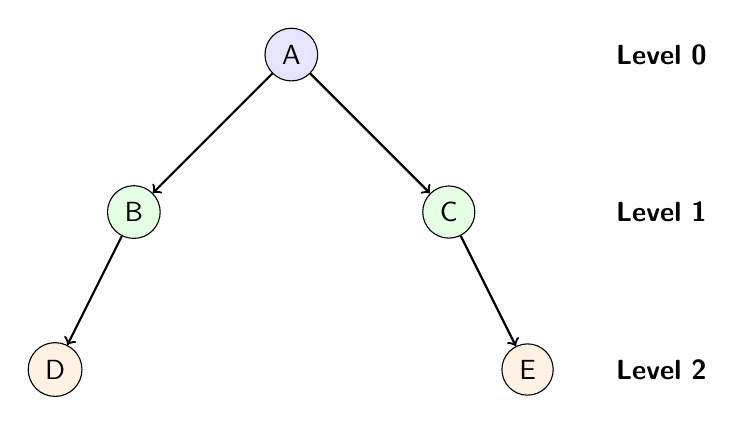
\begin{tikzpicture}[scale=1]
        % Level 0
        \node[circle, draw, fill=blue!10] (A) at (0, 0) {A};

        % Level 1
        \node[circle, draw, fill=green!10] (B) at (-2, -2) {B};
        \node[circle, draw, fill=green!10] (C) at (2, -2) {C};

        % Level 2
        \node[circle, draw, fill=orange!10] (D) at (-3, -4) {D};
        \node[circle, draw, fill=orange!10] (E) at (3, -4) {E};

        % Edges
        \draw[->, thick] (A) -- (B);
        \draw[->, thick] (A) -- (C);
        \draw[->, thick] (B) -- (D);
        \draw[->, thick] (C) -- (E);

        % Level labels
        \node[anchor=west] at (4, 0) {\textbf{Level 0}};
        \node[anchor=west] at (4, -2) {\textbf{Level 1}};
        \node[anchor=west] at (4, -4) {\textbf{Level 2}};
    \end{tikzpicture}
    \end{center}
\end{frame}

\begin{frame}{Analysis of DFS and BFS}
    \textbf{Time Complexity of DFS and BFS:}
    \begin{itemize}
        \item Both DFS and BFS visit each vertex once and each edge once.
        \item Let \( V \) be the number of vertices and \( E \) be the number of edges.

        \item \textbf{DFS Time Complexity:} \( O(V + E) \)
        \begin{itemize}
            \item Each vertex is visited once: \( O(V) \)
            \item Each edge is traversed once: \( O(E) \)
        \end{itemize}

        \item \textbf{BFS Time Complexity:} \( O(V + E) \)
        \begin{itemize}
            \item Each vertex is enqueued and dequeued once: \( O(V) \)
            \item Each edge is traversed once: \( O(E) \)
        \end{itemize}
    \end{itemize}
\end{frame}

% Slide: Next Class
\begin{frame}{Next Class}
    \textbf{Topics:}
    \begin{itemize}
        \item New examples beyond connectivity.
        \item Applications of DFS and BFS in real-world problems.
    \end{itemize}
\end{frame}

\end{document}